%11章,动量
\chapter{动量}
\label{ch:Momentum}

动量动量,就是与运动有关的物理量
\makebox{}\hfill 赵三金如是说

\section*{学习目标}
\begin{todolist}
	\item 理解\gls{momentum}的定义和矢量性质,并求算动量的大小
	\item 了解\gls{impulse}的定义和动量的关系
	\item 掌握并运用\gls{cons momentum}
	\item 解决碰撞的问题,包括碰完之后的粘合
\end{todolist}
\clearpage


\section{动量与冲量}
\label{sec:Momentum and Impulse}
在学习复杂的内容之前,先学习要研究的对象。

\subsection*{动量}
\label{subsec:Momentum}
首先给出动量的定义:
\begin{definition}
A body of mass $m$\si{\kg} and moving with speed $v$ \si{\m\per\s} has momemtum given by $mv$.
\end{definition}

所以,动量就是很简单的,质量与速度的乘积,不过有两点值得注意\\
1.动量是\emph{状态量},意味着,在不同时刻,同一个物体的动量是可能发生变化的。\\
2.动量是\emph{矢量},动量的方向和物体运动的速度方向相同。\\
3.动量的单位是\si{\kg\m\per\s}

\subsection*{冲量}
冲量是物体受到的力与这个力作用的时间乘积,被定义为$\vec{F} \cdot t$ 或者$\int \vec{F} \d t$。 

\begin{TaskBox}
利用国际制单位系统,确定冲量的单位是\si{\N \s}
\tcblower
证明动量单位是\si{\kg\m\per\s}和冲量的单位\si{\N \s}是量纲一致的
\tcblower
两个物理量的量纲一致,这两个物理量会有什么联系?
\end{TaskBox}

\clearpage


\section{碰撞}
\label{sec:Collision}
本章的内容对碰撞和动量守恒的部分浅尝辄止,无需了解太深入的原理,只需要能够利用动量守恒解决碰撞的问题即可。如果想了解更多的话,可以研究ALevel物理

\subsection*{动量守恒}
\begin{theorem}
The total momentum before the impact will always be the same as the total momentum after the impact. Momentum is conserved in an impact given no external forces.
\end{theorem}

\subsection*{碰撞}
因此当两个物体发生碰撞的时候,刚好能够把这两个物体作为一整个系统,恰好能够满足在碰撞发生前和发生后这一段时间内,没有合外力的作用,因此满足动量守恒的要求。
所以对于如下图发生的碰撞,可以利用动量守恒的原理求算碰撞之后的速度分配问题。
\begin{figure}[H]
\centering
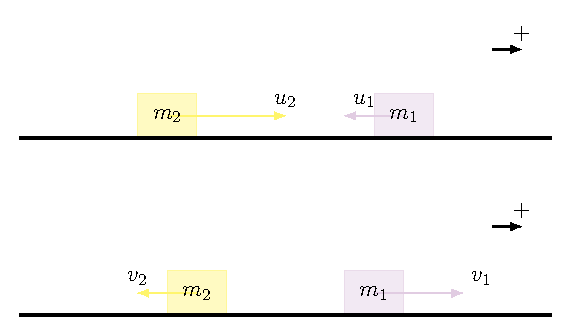
\includegraphics[width=0.8\textwidth]{collision}
\caption{两个发生单一方向碰撞的物体}
\end{figure}

可以写出如下的表达式:
\[
	m_1\overrightarrow{u_1} +m_2\overrightarrow{u_2} =m_1\overrightarrow{v_1} +m_2\overrightarrow{v_2} 
\]
只不过需要注意,动量是矢量,因此要考虑正负方向。


\begin{ExampleBox}
Two snooker balls are travelling towards one another in a straight line when they make a direct impact. Before the impact the first ball had speed $12$\si{\m\per\s} and the second ball had speed $8$\si{\m\per\s}. After the impact both balls have reversed their direction and each has speed $10$\si{\m\per\s} . It is claimed that the balls are not both real snooker balls because they have different masses. Find the ratio of the masses of the balls
\tcblower
理解题意,两个斯诺克台球对向而行,因此取速度较大的那个为正方向,在碰撞之后,两个球的都改变了方向,因此列出动量守恒定律

\begin{align*}
m_1\cdot (+12) + m_2\cdot (-8) &= m_1\cdot (-10) +m_2\cdot (+10)\\
m_1:m_2 &= 9:11
\end{align*}

\end{ExampleBox}
\subsection*{完全非弹性碰撞}
如果碰撞之后,两个物体粘合在一起,以共同的末速度进行运动。这一类的碰撞被我们称之为完全非弹性碰撞。如下图所示
\begin{figure}[H]
\centering
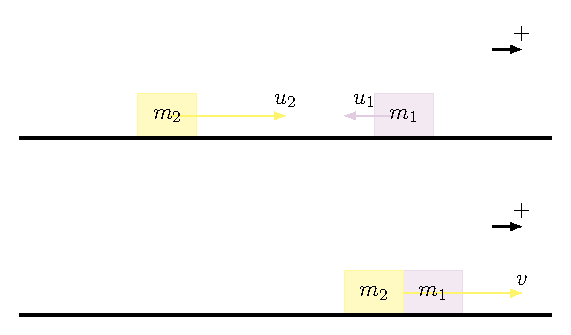
\includegraphics[width=0.8\textwidth]{inela collision}
\caption{碰撞完之后黏在一起}
\end{figure}
对于这样的碰撞,动量守恒的公式会更为简单:
\[
	m_1\overrightarrow{u_1} +m_2\overrightarrow{u_2} =\left( m_1+m_2\right)\overrightarrow{v}
\]
只不过再强调一遍,矢量是有方向的,左右两边都必须是矢量之和,因此对于线性的碰撞,必须明确正负方向,在计算中不能遗漏速度的\emph{正负号}

